\chapter{Introduction and problem statement}
\label{sec_intro1}

Small sample sizes would make wrong or statistically inaccurate conclusions. Therefore, in designing any statistical study, an important step is to estimate the sample size that would enable the researcher to draw valid conclusions. While a small sample size prevents reliable or meaningful statistical conclusions, large sample sizes has rarely been an issue, in fact a large sample size was a desirable aspect of a study. However, in 21st century, having large sample sizes also, becomes a trouble-maker. By emerging technologies that make the task of data collection easy and fast, the size of samples in many studies becomes larger and larger, and this came to the point that, the power of a typical computer would fail to analyze such huge datasets. 

There are several issues related to a large datasets, including: how to store them, how to load them, and how to analyze them. Our interest in this thesis is in the last one. Although the last issue, the same as the two others could be solved using ideas coming from computer science, or simply, increasing the computation power of the hardware we use could solve the issue, we believe statistical methods and ideas can provide solutions that are easy to understand, capable of being implemented in different situations, and also accurate. This becomes more important when we realize increasing the computation power and size of available datasets are highly and positively correlated. 

In Table \ref{tab_comptime1} we compare the computation when the sample sizes $n=10, 10^2, 10^3, 10^4, 10^5, 10^6, 10^7$, for some simple computational tasks including:

\begin{itemize}
\item Generating a random sample from standard normal of size $n$.
\item Finding the mean of the generated sample.
\item Finding the variance of the generated sample.
\item Fitting a linear model to the generated sample as the predictor and $y = 1 + ex + \epsilon$, where $\epsilon\sim N(0, 0.01)$.
\item Fitting a MAD (mean absolute deviation) regression to the same data.
\end{itemize}



\begin{table}[ht]
\centering
\begin{tabular}{lccccc}
  \hline
Sample size & Generating a normal sample & Mean & Variance & Linear model & MAD regression \\ 
  \hline
 10.00 & 0.00 & 0.00 & 0.00 & 0.00 & 0.00 \\ 
 100.00 & 0.00 & 0.00 & 0.00 & 0.00 & 0.00 \\ 
 1000.00 & 0.00 & 0.00 & 0.00 & 0.00 & 0.00 \\ 
 10000.00 & 0.00 & 0.00 & 0.00 & 0.00 & 0.06 \\ 
 100000.00 & 0.00 & 0.00 & 0.00 & 0.01 & 3.75 \\ 
 1000000.00 & 0.08 & 0.01 & 0.00 & 0.32 & 764.37 \\ 
 10000000.00 & 1.05 & 0.01 & 0.06 & 3.46 & 60558.83 \\ 
   \hline
\end{tabular}
\caption{Computation time (in seconds) of different methods for different sample sizes.} 
\label{tab_comptime1}
\end{table}



As we may see, for some analyses, the computation time increases linearly as the sample size increases, but for others, it would even speeds down with a sub-linear rate. Once the cause of expensive computation time is the sample size, an effective solution could be to split the very large sample into smaller sub-samples and then analyze them separately. As each sub-sample has a smaller size, and analyzing these different sub-samples are independent of each other (can be run in parallel), the overall computation time can be decreased. 

Splitting a sample into smaller chunks, then analyzing each part separately, and finally combine the results of these analyses is a known methodology to deal with large samples. Some authors have called this \emph{Software Alchemy}, \cite{matloff2014}. This idea is also at the heart of MadReduce methodology \citep{dean2008}. The split-apply-combine strategy in the R packages {\tt{plyr}} and {\tt{dplyr}} also uses this idea \citep{wickham2011}. All these would show the importance of this approach. Furthermore, Figure \ref{fig_bigdata} shows a plot of number of results found using Google scholar when searching the exact phrase "big data" upto different years. We obviously can see the increasing interest in the topic in the recent years.




\begin{figure}
\centering
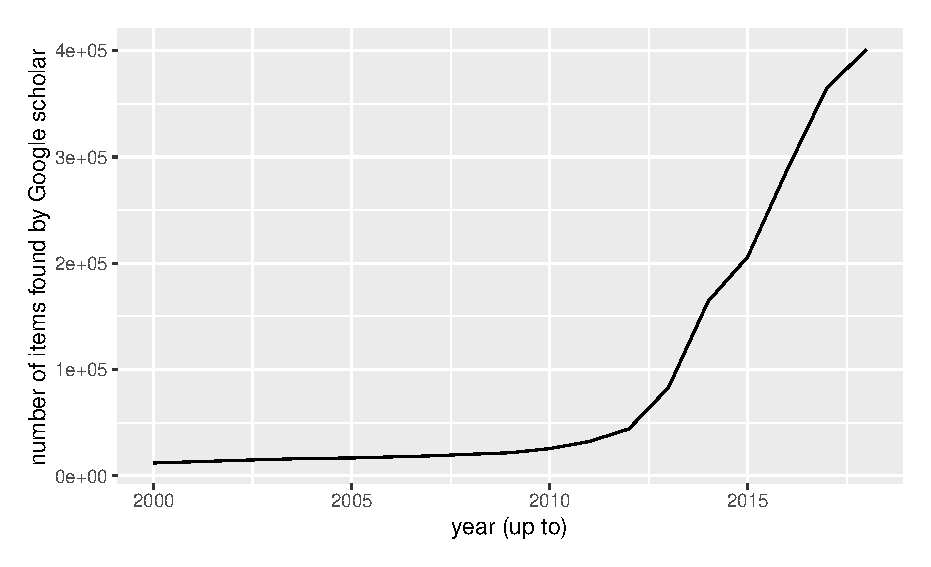
\includegraphics[width=\textwidth]{bigdata.eps}
\caption{Number of items found by Google scholar when searching the exact phrase "big data" up to different years.} 
\label{fig_bigdata}
\end{figure} 




However, most of these implementations would consider independent sub-samples, or non-clustered data. Our goal in this thesis to extend the existing methodology to the cases where the subjects would form clusters of correlated data. This type of data is very common in medical studies in particular, but they also can be observed in any longitudinal or multilevel study. Some examples of such data are measurement on offsprings of the same animal. Data collected from family members. Data collected from different countries in a meta-analytic setting. Measuring body temperature of the same person several times, ratings of the same book by different people, measuring hearing ability of elderly people for several frequencies, measuring primary vital signs (body temperature, heart rate, respiratory rate, and blood pressure) for each person, etc.

As we have seen in Table~\ref{tab_comptime1}, even for non-clustered data and simple models, increasing the sample size could cause very expensive computation times. The time needed to fit a MAD regression with one predictor to a sample of size 10 million is around 18 hours. Now, if we have clustered data that needs more complicated models, things would get even more difficult. In case of clustered data, the sample size can be seen from different angles. 





\section{Large clustered data}

Consider a study which measures (at most) $m$ outcomes for $N$ clusters, each $n_i$ times. Let $y_{rij}$ be the $j$th measurement taken on the $i$th cluster for the $r$th outcome, $i=1,\ldots,N$, $r=1,\ldots,m$ and $j=1,\ldots,n_{ri}$. As a simple example, take $m=4$ responses as the vital signs: body temperature, heart rate, respiratory rate, and blood pressure, measured for $n_1 = n_2 = n_3 = n_4 = 100$ hospitalized patients. And assume these measurements are done every $4$ hours. So, $y_{111}$ is the body temperature of the first patient measured for the first time). 

A general scheme of such clustered data is presented in Figure~\ref{fig_scheme}. A suitable model for such data should appropriately respect the correlation structures imposed by the fact that several measurements are done on the same subject. While even for moderate sample sizes, fitting such models could already become challenging, we may face a greater challenge when the size of dataset makes it eligible for the title \emph{big data}. 

\begin{figure}
\centering
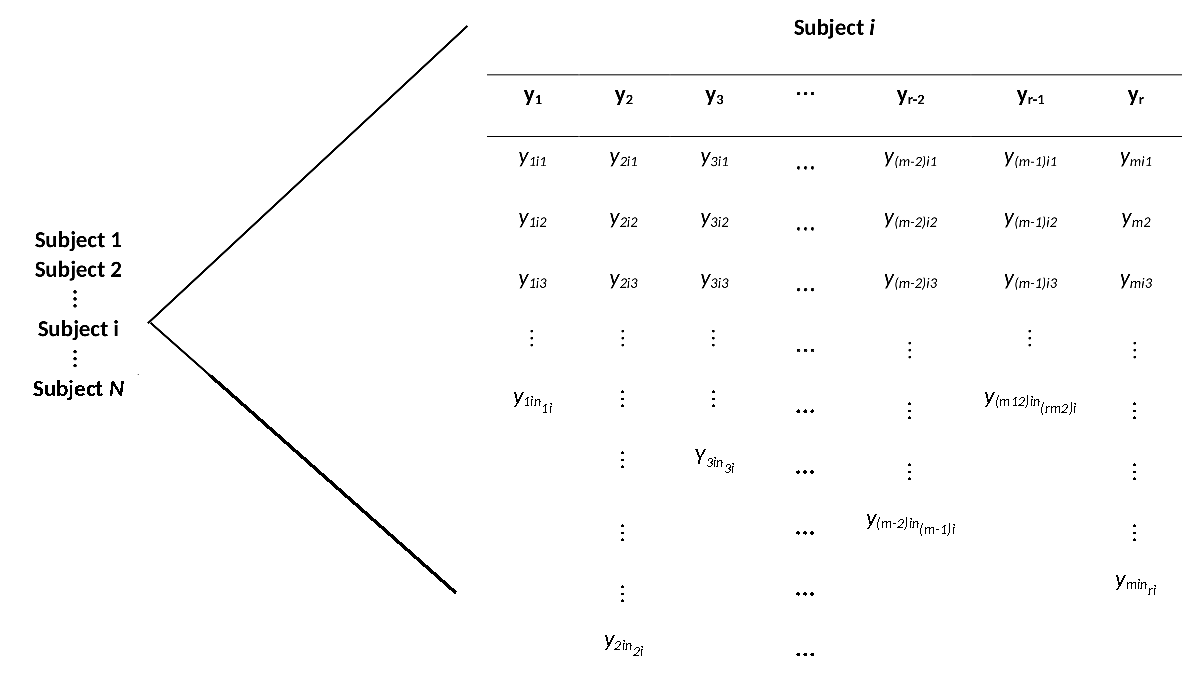
\includegraphics[width=\textwidth]{scheme_new.eps}
\caption{General scheme of the clustered data we consider through this thesis.} 
\label{fig_scheme}
\end{figure} 


As it was mentioned, for non-clustered data big would mean a large number of subjects. However, in our case, a dataset could be entitled as \emph{big data} in different situations. In case of the clustered data of interest in this thesis, data are considered to be big if at least one of the following applies:
\begin{itemize}
\item When the sample size, $N$, becomes very large,
\item When the cluster sizes become very large:
\begin{itemize}
\item When the number of measurements per outcome for some clusters, $n_{ri}$'s, becomes very large,
\item When the number of outcomes, $m$, becomes very large.
\end{itemize}
\end{itemize}

Note that, \emph{big} would be different for $N$, $n_{ri}$, and $m$. For example, in case of a MAD regression, we have seen a dataset of size $N=100,000$ could be analyzed in $0.001$h, increasing the sample size to $N = 1000,000$ would increase the computation time to $0.2$h, which is not fast, but still feasible, but $N=10,000,000$ would take around $17$ hours which could be too much. Therefore, in the case of a simple MAD regression, we may consider $N>10,000,000$ as \emph{big}.

When it comes to clustered data, however, there is a different story. Some 100's could already be big in case of cluster size, $n_{ri}$ (see Amazon book ratings data ({\bf{give reference to the section}})), and even some 10's is \emph{big} when we consider the number of outcomes $m$ (see Hearing data)({\bf{give reference to the section}}).

It goes without saying that, in reality, any combination of the above situations could happen. Our aim in this thesis to provide appropriate methodology to: 1- split the data into smaller chunks, 2- analyze each split, 3- combine these analyses in an efficient way. Our methodology should consider the nature of the data. While the mere task of splitting would already breaks down the difficult (sometimes infeasible) problem into smaller easier and feasible to analyze pieces, sometimes the structure of the data would allow for some \emph{smart} other than random splitting which would then provide more gain. Our aim in this thesis is to cover all of the situations which a dataset of clustered subjects could be called \emph{big}. We will go over our proposal for splitting/analyzing/combining steps for each of these cases. 

In developing these methodologies we will make sure to keep two promises:

\begin{itemize}
\item While each methodology can deal with one situation, it should be easily possible to combine methodologies to deal with a combined situation.

\item The splitting and combining steps of our methodology should be as independent as possible from the analyses step, so one can easily (or with a minor modification) use it for its desired analysis.
 
\end{itemize}

\section{Data splitting: a unified approach}

Data splitting is a general idea to deal with big, massive, and large data. Large here could be called to any of the cases we have mentioned above, or a combination of them. Our general approach to deal with this situation consists of three main steps which we would call them together Data splitting.

\begin{enumerate}
\item \textbf{Splitting}: in this step, the data should be splitted into smaller chunks in a way that analyzing each of them becomes more convenient that the dataset as a whole. This convenience would at least come from having sub-samples of smaller sizes, but it could be possible to perform the splitting in a way that some other nice features (balancedness, for example) that the original data does not own, can be created in all or some of these sub-samples.

2- \textbf{Analyzing}: in this step, each split of data will be analyzed using the conventional methods. Therefore, using \emph{data splitting} approach, one can use its own favorite methodologies which are only suitable for small to moderate sample sizes. Typically, with \emph{data splitting} approach, the only information one needs to extract and keep from analyzing each split of data are: the estimated parameter vector, and their covariance matrix (if there is a need to provide standard errors of such estimates).

3- \textbf{Combining}: within this unified framework, each parameter in the model could be estimated several times. As our interest is to have one single set of parameter estimates, the last step in this paradigm is to combine all of analysis results from the second step into one single set. This should be done via appropriate combination rules. The combination rule is simply a weighted average of the results from different splits. Therefore, there is the need for proposing appropriate weights. Also, when it comes to combine covariance matrices, the fact that these results are coming from different (possible dependent) sub-samples should be well respected. 

\end{enumerate}



In the following sections we will review different splitting approaches, also their appropriate combination rules. WE will also give examples of our motivating datasets where each of these approaches could be beneficial. 

\section{Different types of splitting}

We have already discussed the MapReduce, or split-apply-combine approaches. The main splitting technique that is implemented using such approaches is to split the data: 1- randomly, 2- at subject level. Throughout this these we would call the splitting at the subject level \emph{horizontal splitting}. The reason for that can be seen in the Figure~\ref{fig_scheme}. If we illustrate the splits by separating lines, such lines will be horizontal. On the other hand, if the splitting is done for the data within a subject, then the lines should be drawn vertically. This case is specific to the clustered data where we have more than one observation for each subject. 

While random splitting (assigning members of each split at random) is an effective way in many situations, there are cases where assigning members of each split based on a predefined structure has an added value. We call such splitting approach structural splitting as opposed to random splitting. In the following we will give an overview of the four types of splitting, and present examples where each of them could be useful. We will also briefly go over analyzing and combining steps also.

\subsection{Random horizontal splitting}    

Random horizontal splitting, as its name suggested tries to assign different subjects to different splits at random. There are several ways to do this task, the way we have used in our implementations is as follows, for a sample of size $N$,

\begin{enumerate}
\item To split the dataset into $M$ sub-samples, take $m = [{N/M}]$ as the size of each split to make sub-samples of roughly the same sizes.
\item Generate a random sample of size $N$ from standard normal.
\item Order the generated sample.
\item Divide the ordered indexes into (M-1) parts of size $m$, and the $m$th chunk will include all the remaining indexes. These will be the index of subjects that should be assigned to each split.
\end{enumerate}

Note that, $M$ should be carefully selected. Two main points to consider when selecting $M$ are first to make sure the resulting sub-samples are small enough to keep the computation time at an acceptable level, but at the same time one needs to be careful that the sub-samples stay large enough, so the methodologies can still be applied on them in a valid way.

Assume $\widehat{\theta}_1, \ldots, \widehat{\theta}_M$ are the estimated parameters from $M$ sub-samples, the data splitting estimate of this parameter can be computed as follows:

\begin{equation}
\label{eq_estimate}
\widetilde{\theta} = \sum_{m=1}^M \widehat{\theta_m},
\end{equation}
where $\sum_{m=1}^M w_m = 1$. An appropriate weights could be assigned proportional to the size of each split. We would call such weights proportional weights in this thesis:

\begin{equation}
\label{eq_prop_w} 
w_{prop, i} = \frac{m_i}{N}.
\end{equation}

Of course, in case of random splitting, as the split sizes are roughly the same, one can simple assign equal weights to different sub-samples. Such weights are called equal weights in this thesis:

\begin{equation}
\label{eq_equal_w}
w_{equal,i} = \frac{1}{M}.
\end{equation}

The combination rule in case of horizontal splitting is simpler than vertical splitting. This comes from the fact that the sub-samples are independent in this case, therefore, one does not need to be concerned about the correlations between the estimates coming from different sub-samples. For a general weight $w_i$, consider $\mathrm{Var}(\widehat{\theta}_i) - \sigma^2_i$, then the variance of data splitting estimator can be computed as follows:

\begin{equation}
\label{eq_variance1}
\mathrm{Var}_{horizontal}(\widetilde{\theta}) = \sum_{m=1}^M w_m^2 \sigma_m^2.
\end{equation}

As having a smaller variance is a desired property for an estimator, Equation (\ref{eq_variance1}) would give an idea about an alternative way of assigning weights to our estimates: the weights should be computed in a way that the variance in (\ref{eq_variance1}) becomes minimized. In this thesis, such weights are called optimal weights. We define the optimal weights as the minimizer of the following objective function:

\begin{equation}
\label{eq_objective_opt_w}
Q = \sum_{m=1}^M w_m^2 \sigma_m^2 - \lambda \left(\sum_{m=1}^M w_m -1 \right),
\end{equation}

where $\lambda$ is a Largange multiplier to make sure that the sum of estimated optimal weights is still 1. Solving the optimization problem in (\ref{eq_objective_opt_w}) would lead to the following optimal weights,

\begin{equation}
\label{eq_opt_w}
w_{opt, i} = \frac{1/\sigma^2_i}{\sum_{m=1}^M 1/\sigma^2_m},
\end{equation}

As one may see, we may give more weights to a sub-sample with smaller variance.


In using optimal weights, one needs to be concerned about the fact that, optimal weights are including parameters from model, which then needs to be replaced by an estimate (we will discuss different ways of doing it in the coming chapters), and these estimates will come with their own variability. So, if the variability these estimates will bring together with them becomes larger than the variability that the optimal weights could decrease, then it is better to use the simpler parameter-free weights.

An example in our motivation datasets that random horizontal splitting can be beneficial is the Divorce in Flanders dataset, where clusters are formed by family members. While each family is at most of size 7, the number of total available families is large enough to make conventional software to fail. By splitting this large sample randomly and at the family level (horizontally), we could be able to fit the models and answer the research questions.

\subsection{Structured horizontal splitting}

As we have discussed, random horizontal splitting has been used by many researchers in different contexts to deal with big data issue. However, a randomly horizontal split would only decrease the sample size. So all of our gain is due to having smaller sample sizes. We have observed that they are cases where splitting using a pre-defined structure would provide some added benefits on top of just having smaller sub-samples.

It is a well-known fact that a balanced study deign works better than an unbalanced one. By balanced we mean, the number of available data for each cluster is the same. In fact, most of the studies are planned to be balanced, but in practice they would rarely end up like that. One can see several reasons for that, for example, the required materials are not enough, some patients die, some animals fail to follow the instructions, etc. Therefore, while having a balanced set of data is desired and even planned, we will usually have an unbalanced data to analyze. 

Although most of the data in practice are unbalanced, one can usually find balanced sub-sets of those data. Take our example on a developmental toxicity study. There, the clusters are made of fetuses within litters. Obviously, different mothers would have different number of babies: an inevitably happened unbalanced data. However, it is not like that the number of fetuses within litter from every single mother is different from the others. Table \ref{tab_litter_size} shows unique number of fetuses in different litters with their frequencies. As one may see, we have a limited number of cluster sizes. Therefore, although the complete data is unbalanced, it is formed by balanced sub-sets. An structured horizontal splitting would assign all clusters of the same size to one sub-sample. 


\begin{table}[ht]
\centering
\label{tab_litter_size}
\caption{Unique cluster sizes and their frequency in a developmental toxicity case study for the response DEHP.}
\begin{tabular}{lcccccccccccc}

  \hline
Cluster size & 9 & 10 & 15 & 8 & 12 & 13 & 14 & 6 & 7 & 3 & 11 & 16 \\ 
  Frequency & 10 & 9 & 3 & 12 & 20 & 18 & 6 & 4 & 5 & 4 & 9 & 4 \\ 
   \hline
\end{tabular}
\end{table}

As it was mentioned, there are several benefits for a balanced dataset, and in the special case of clustered data, we have shown that a closed-form solution exists when the cluster sizes are balanced, whereas for unbalanced data one needs to fit the models using iterative procedures. For very large datasets, the iterative procedures could be prohibitive and slow. While, a closed-form solution can be computed much faster. We have observed tens of thousands time faster computation using structured horizontal splitting based on the cluster sizes. Two cases are studied in details: clustered data with a compound-symmetry (CS) covariance structure, and clustered data with an autoregressive of order 1 (AR1) covariance structure. It worth to note that, even if the closed-form does not exist, with a balanced dataset one would have a faster and more stable convergence compared to unbalanced data.

The two considered covariance structures would cover a wide range of applications: where the correlation between to  members of a cluster is always the same (compound-symmetry), and when it decreases when the distance between the two observations becomes larger (AR1). For these two cases, the existance of the closed-form solution are shown using sufficient complete statistics. Then these closed-form solutions are obtained, also various kinds of weights, including optimal weights are computed for each case. On top of the already discussed weights, as we have clusters of all different sizes in each sub-sample here, we have proposed another type of weights, as follows,

\begin{equation}
\label{eq_size_prop_w}
w_{size-prop, i} = \frac{m_i n_i}{\sum_{k=1}^ M m_k n_k},
\end{equation}

In some cases that the cluster size is also important (other than the number of subjects in each sub-sample), such weights would perform better. We have shown that AR(1) is one of these cases, while for the CS, proportional weights would work fine. 

Note that, the structured horizontal splitting idea is very general and all the introduced methodologies regarding different weights, combination rules, etc., can be used for any suitable structure of splitting (as long as they are horizontal), but in this thesis we only consider the cases where the structure is defined based on size of the clusters. 

\subsection{Random vertical splitting}

The horizontal splitting techniques that we have introduced and discussed so far would be beneficial when the number of clusters ($N$) is large, but the cluster size is still small or moderate, so by breaking down the large $N$ into $M$ smaller sub-samples, we can manage to solve our problem. But there are examples where the size of some or all of the clusters is also very large. And as we have mentioned, large for a cluster size has a much smaller magnitude compared with large for the number of clusters. In such cases, horizontal splitting would not help much, because each cluster in our sub-samples is still large, so by horizontal splitting we just breakdown one problem into $M$ problems. 

As n example, take the Amazon book ratings. There, we have the ratings for many books given by different buyers. Therefore, each book could possibly be rated by thousands of people. This will for very large clusters where even the simple models would fail to converge. In such a case, horizontal splitting cannot solve our problem. To solve the issue here, we have to perform the splitting within the subject. For example, if there are 5000 people rating a book, in order to make smaller clusters in our sub-samples, we have to split these 5000 people, e.g., into 100 sub-samples, each of size 50. 

As long as the interest is in the parameter estimate, the combination rules in (\ref{eq_estimate}) is still valid. But the difficulty will appear in deriving the combination rule for the variances. As the data from different clusters are shared among different sub-samples, in other words, one cluster is present in more than one sub-sample, the estimated parameters from different sub-samples are correlated, and obviously, when combining the variances, these correlations should be taken into account. 

One way to deal with the combination rule of variance in case of vertical splitting is to look at our sample splitting based model fitting in the pseudo-likelihood methodology, rather than the likelihood. In fact, once the dataset is analyzed in whole we use the conventional likelihood theory by finding the estimate of our parameters by maximizing the likelihood function. But when the data is splitted into some sub-samples, each of these sub-samples are analyzed using a likelihood theory, but their combination is not the original likelihood function anymore. It is called pseudo-likelihood. Roughly speaking, pseudo-likelihood theory tries to replace the complex or difficult likelihood function with something simpler or easier. But maximizing both likelihood or pseudo-likelihood functions would follow the same goal, i.e., estimate the same set of parameters, but with different precision.

From Cram\'{e}r-Rao's lower bound we know that the lower bound for variance can be achieved by a maximum likelihood estimator. In other words, any other estimator (including maximum pseudo-likelihood) would come with a variance larger than the one from a maximum likelihood. Therefore, having the easier problem to solve comes at the price of losing a bit of accuracy. 

Let us define the pseudo-likelihood in plain English. Assume we have a sample $\mathbf{y}$ and using that we want to estimate the parameters vector $\theta$ via the log-likelihood function $\ell(\theta; \mathbf{y}$. Via sample splitting, we split the sample $\mathbf{y}$ into $M$ sub-samples $\mathbf{y_1}, \ldots, \mathbf{y_M}$, then feed them to the same likelihood function and estimate the parameter vector $\theta$ $M$ times. Under pseudo-likelihood paradigm, one can look at this as estimating a parameter vector $\Theta = (\theta_1, \theta_2, \ldots_3, \theta_M)$ using the sample $\mathbf{Y} = (\mathbf{y_1}, \ldots, \mathbf{y_M})$ via maximizing the pseudo-likelihood function $p\ell(\Theta, \mathbf{Y})$. Note that, $\theta_1 = \theta_2 = \theta_3 = \ldots = \theta_M$. 

Now that the problem is defined under a pseudo-likelihood theory, all the results obtained there can be carried over to the data splitting as well. If we consider matrix $A$ that combines the estimates, i.e., $\widetilde{\theta} = A\widehat{\Theta}$, then the most important result we can present is:

\begin{equation}
\label{eq_clt_pseudolikelihood}
\sqrt{N}(\widehat{\theta} - \theta) = \sqrt{N}(A\widehat{\Theta} - A\Theta) \stackrel{d}{\sim} N\left(\mathbf{0}, A I_0^{-1} I_1 I_0^{-1} A^{T}\right),
\end{equation}

where $T$ means the transpose, and $I_0$ and $I_1$ are defined as follows,
\begin{equation}
\label{eq_hessian_gradient_pl}
I_0(\Theta) = \mathrm{E} \left(\frac{\partial^2 p\ell(\Theta; \mathbf{Y})}{\partial \Theta^T \partial \Theta} \right),\; I_1(\Theta) = \left[\left(\frac{\partial p\ell(\Theta)}{\partial \theta} \right)^T \frac{\partial p\ell(\Theta)}{\partial \theta}  \right].
\end{equation}

More details on pseudo-likelihood interpretation of the data splitting can be found in \cite{Iddi2011}. However, a main difficulty to find the variance in (\ref{eq_clt_pseudolikelihood}) if the need to cluster-wise hessian and gradient of the pseudo-likelihood function. This could easily become expensive. Another difficulty with this approach comes from the fact that, depending on the derivative and hessian means this variance estimator needs to computed case by case. For example, the results obtained for a logistic regression cannot used for another model without the necessary modification. To overcome these difficulties, we have considered an alternative solution proposed by \cite{hoffman2001} in different context. Their approach is called within cluster re-sampling, which was later on extended and renamed to \emph{multiple outputation} by \cite{follmann2003}.

In order to explain the motivation behind the multiple outputation technique, consider clustered data where the cluster consists of blood pressure of a patient visiting a hospital several times. The objective of the study is the severity of a disease which is highly correlated with blood pressure (more severe the disease, the larger the blood pressure). As the blood pressure is measured every time the patient is visiting the hospital, a larger cluster size, means the patient has visited the hospital more, which itself means the patient had more issues with the blood pressure, so a more severe state of the disease. In other words, in such situations the size of the cluster is also correlated with the response and objective of the study. Such situations are also called \emph{informative cluster size} in the literature. The correlation of cluster size and the response should be respected in the model, otherwise it could cause issues. Multiple outputation has been proposed to deal with this problem.

Within cluster resampling proposed by \cite{hoffman2001} to deal with the so-called informative cluster size, when it is a nuisance parameters, i.e., we are not interested to study the correlation of the response and cluster size, we just want estimates of other parameters which are not affected by this correlation. \cite{hoffman2001} proposed to take sub-samples of size 1 from each cluster repeatedly to form a sample on non-clustered data every time. Then the conventional methods can be used for each of these non-clustered data. The results then can be combined via combination rules which are similar to (\ref{eq_estimate}) for the estimates. But for the variance \cite{hoffman2001} proposed the following combination rule:

\begin{equation}
\label{eq_combination_variance}
\mathrm{Var}(\widetilde{\theta}) = W - \left(1 + \frac{1}{M}\right) B,
\end{equation}
where $W$ and $B$ are within and between sub-samples variances respectively. These quantities are defined as follows,
\begin{equation}
\label{eq_W_B_Var}
W = \frac{1}{M} \sum_{i=1}^M \sigma^2_m,\; B = \frac{1}{M-1} \sum_{i=1}^M \left(\widehat{\theta}_i - \widetilde{\theta} \right)^2.
\end{equation}

As one may see, the combination rule for the variance in (\ref{eq_combination_variance}) is also intuitively interesting also. It states, the variance of the data splitting estimator is an average of the variance in different sub-samples, but when we subtract it from the sample variance of estimated parameter from different sub-samples. Looking at this combination rule, one might also understand the reason behind naming this method multiple outputation by \cite{follmann2003}. That comes with various similarities of this technique with multiple imputation. Although, the similarities are technically rather than literally. 

First let us say a word on multiple imputation itself. Multiple imputation (MI) is an effective way to deal with missing data issue. The traditional missingness remedies would try to either ignore that missing part of the sample, or replace it with a single plausible value. This way, one would treat a missing before and now imputed value the same as a value which is originally observed. In order to respect the fact that imputed values are actually imputed and as well could be any other value, \cite{rubin1978} proposed to replace each missing value with several values and not just one single value. 


Now we may look at similarities of MI and MO. As it was mentioned, multiple imputation creates artificial data and augment it to the incomplete sample to make it complete, on the contrary, but in a similar way, multiple outputation would every time put some part of the same out of the analysis. Therefore, multiple \textbf{im}putation increases the sample size by including new artificial data, while multiple \textbf{out}putation decreases the sample size by selecting only a subset of them. But in both of the methods, we will have several datasets to analyze rather than the one single original dataset. So, in both methods we estimate each parameter several times. This is also reflected in the variance estimator. Let us remind the combination rule for variance from \cite{rubin1987},

\begin{equation}
\label{eq_comb_var_MI}
\mathrm{Var}(\widehat{\theta}_{MI}) = W + (1 + \frac{1}{M}) B.
\end{equation}

As one may see, the only difference of (\ref{eq_comb_var_MI}) and (\ref{eq_combination_variance}) is in the fact that MI would add the between datasets variability of the estimated parameter to the averaged variance, while MO would subtract this. And intuitively, that would also make sense, in case of MI we artificially increase the sample size, so we would get a smaller variance which needs a correction (to become larger, as it should be), but in case of MO we decrease the sample size, so a larger variance would be obtained, which is the also corrected in the same was as MI just with a different sign.

Because of the discussed similarity and for the vast use of multiple imputation in practice, we have developed part of contributions with the target to be used in data splitting for the case of multiple imputation. As for many cases, the conclusions and results from MI are also valid for MO, and vice versa. 

We have extended the idea in within cluster re-sampling and multiple outputation to it them suitable for our purpose: analyzing clustered data with big clusters. The so-called iterative multiple outputation (IMO) procedure is proposed to fulfil this role. IMO is proposed as follows,

\begin{enumerate}
\item \textbf{Start.} Select an initial number of sub-samples, $M_0$, and sub-sampling size $m$. Take $M_0$ sub-samples of size $m$, fit the model to each and obtain $\widehat{\theta}_i$ and its variance $\Sigma_{\widehat{\theta}_i}$ ($i=1,\ldots,M_0$). Then compute 
\begin{equation}
\label{comb_rules}
\widetilde{\bftheta}_{M_0} = \sum_{i=1}^{M_0} \widehat{\bftheta}_i,\;\; \Sigma_{\widetilde{\theta_{M_0}}}=\widehat{W}_{M_0} - \left( \frac{M_0+1}{M_0} \right) \widehat{B}_{M_0}.
\end{equation}

			\item \textbf{Update.} For $m>M_0$, \begin{equation}
	\label{update}
	\widetilde{{\bftheta}}_{m+1}=\frac{m\widetilde{\bftheta}_m + \widehat{\bftheta}_{m+1}}{m+1},\; \Sigma_{\widetilde{\theta}_{m+1}}=\widehat{W}_{m+1} - \left( \frac{m+1}{m} \right) \widehat{B}_{m+1}.
	\end{equation}
	\item \textbf{Distance.} Compute: $d_{m+1}=d(\widetilde{\bftheta}_{m+1},\widetilde{\bftheta}_{m})$ using an appropriate distance.
	\item \textbf{Stopping rule.} $d_{j} < \varepsilon$ for $j=m+1,\ldots,m+k_0$.
\end{enumerate}
Where for $m=r$ we have,
\begin{equation}
\widehat{W}_r= \frac{\sum_{i=1}^r \sigma_{\widehat{\theta}_i}}{r},\; \widehat{B}_r= \frac{\sum_{i=1}^r (\widehat{\theta}_i - \widetilde{\theta}_r)(\widehat{\theta}_i - \widetilde{\theta}_r)'}{r-1}.
\end{equation}

We may remark that, there are cases only $M=1$ sub-sample would be sufficient to obtain results almost as efficient as analyzing the full dataset. We have studies this matter in detail and called such estimators \textit{finite information limit estimators}. We have also proposed procedures to detect this property.

A very useful dataset to illustrate the usefulness of random vertical splitting is the Amazon's book ratings dataset. This set of data consists of ratings of several books (from 1 to 5) on Amazon website. Each book is rated by different number of people, which could be as small as 1 and as large as 20,000. So we will deal with clustered data of very variable and large sizes. 


\subsection{Structured vertical splitting} 

So far we have discussed random horizontal and random vertical splitting, as well as structured horizontal splitting. In case of the vertical splitting also, pre-defining some structures to take the sub-samples other thank taking them just at random could be beneficial. We have already seen one application of structured splitting in case of horizontal splitting, which enabled us to form balanced sub-samples. Defining an structure is not always for computation efficiency. Sometimes, without such structure, estimating the model parameters is not possible. 

We have considered an important case of jointly modeling several outcomes via random effects as a useful example for structured vertical splitting. Such a problem can easily become infeasible when the number of outcomes becomes large (even tens of them). \cite{fieuws2006, fieuws2007} proposed to analyze all possible pairs of all outcomes instead of analyzing them simultaneously. Then use appropriate combination rules to find the parameters of the model of interest. To illustrate the problem, also to show how structural vertical splitting is similar to the approach of \cite{fieuws2006, fieuws2007}. Also, to see how it is different from random vertical splitting, we present a simple example. 

Imagine we have 3 outcomes to be jointly modeled. A random effects approach would fit a separate model to each outcome, then let them to be correlated by defining a joint distribution for their random effects. This joint distribution is usually a normal distribution where its covariance matrix would capture the dependencies between different outcomes. Let us elaborate more here, if the three separate models (all linear) for the three outcomes are defined using the following general form:

\begin{equation}
\label{eq_SV_models}
\begin{cases}
y_{1ij} = \beta_1 + b_{1i} + \epsilon_{1ij} \\
y_{2ij} = \beta_2 + b_{2i} + \epsilon_{2ij} \\
y_{3ij} = \beta_3 + b_{3i} + \epsilon_{3ij},
\end{cases}
\end{equation}
we let the three random intercepts to be normally distributed as follows,
\begin{equation}
\label{eq_SV_D}
\begin{bmatrix}
b_{1i} \\
b_{2i}\\
b_{3i}\\
\end{bmatrix} \sim N \left ( 
\begin{bmatrix}
0 \\
0\\
0\\
\end{bmatrix}, 
D=\begin{bmatrix}
D_{11} & D_{12} & D_{13}\\
 & D_{22} & D_{23}\\
&& D_{33}\\
\end{bmatrix}
\right).
\end{equation}
Therefore, the parameter of interest, $\bftheta$, is as follows:
\begin{equation}
\label{eq_SV_theta}
\bftheta= (\beta_1,\beta_2,\beta_3, D_{11},D_{22},D_{33},D_{12}, D_{13}, D_{23}).
\end{equation}
As we have $3$ outcomes, the number of pairs will be $M=3\times (3-1) /2 =3$. However, unlike random vertical splitting where usually all parameters of interest are estimated in each sub-sample, here, because of the special structure we have imposed on the sub-samples, each of them would estimate part of parameter vector. The parameters estimated in each pair ($\bftheta^{(s)}$) are as follows:
\begin{equation}
\label{eq_SV_pairs}
\begin{cases}
\bftheta^{(1)}=\theta_{(y_{1ij},y_{2ij})} = (\beta_{1_1},\beta_{2_1},D_{11_1},
,D_{22_1},D_{12_1}) \\
\bftheta^{(2)}=\theta_{(y_{1ij},y_{3ij})} = (\beta_{1_2},\beta_{3_2},D_{11_2},
,D_{33_2},D_{13_2}) \\
\bftheta^{(3)}=\theta_{(y_{2ij},y_{3ij})} = (\beta_{2_3},\beta_{3_3},D_{22_3},
,D_{33_3},D_{23_3}),
\end{cases}
\end{equation}
as one may see in (\ref{eq_SV_pairs}), each $\bftheta^{(s)}$ ($s=1,2,3)$ is a subset of $\bftheta$ in (\ref{eq_SV_theta}. Now, the stacked vector combining all parameters estimated in different sub-samples $\boldsymbol{\Theta}'=(\bftheta^{(1)},\bftheta^{(2)},\bftheta^{(3)})$ can be constructed as follows:
\begin{equation}
\label{eq_SV_Theta}
\boldsymbol{\Theta}'=(\beta_{1_1},\beta_{2_1},D_{11_1},
,D_{22_1},D_{12_1}, \beta_{1_2},\beta_{3_2},D_{11_2},
,D_{33_2},D_{13_2},\beta_{2_3},\beta_{3_3},D_{22_3},
,D_{33_3},D_{23_3}).
\end{equation}
As one may see, the covariance parameters ($D_{12},D_{13}, D_{23}$) are only estimated once using their corresponding pair, but the rest of parameters are appearing in two out of three pairs. Therefore, to combine these estimates we cannot just average all estimates as we did in (\ref{eq_estimate}). The weight matrix to perform the appropriate combination can be defined as follows,
\vspace*{2mm}
\renewcommand{\kbldelim}{(}% Left delimiter
\renewcommand{\kbrdelim}{)}% Right delimiter
% \resizebox{\textwidth}{!}{  
\[
  A = \kbordermatrix{
    & \beta_{1_1}&\beta_{2_1}&D_{11_1}
	&D_{22_1}&D_{12_1}& \beta_{1_2}&\beta_{3_2}&D_{11_2}
	&D_{33_2}&D_{13_2}&\beta_{2_3}&\beta_{3_3}&D_{22_3}
	&D_{33_3}&D_{23_3} \\
\beta_1 & 1 & 0 & 0 & 0 & 0 & 1 & 0 & 0 & 0 & 0 & 0 & 0 & 0 & 0 & 0 \\ 
  \beta_2 & 0 & 1 & 0 & 0 & 0 & 0 & 0 & 0 & 0 & 0 & 1 & 0 & 0 & 0 & 0 \\ 
  \beta_3 & 0 & 0 & 0 & 0 & 0 & 0 & 1 & 0 & 0 & 0 & 0 & 1 & 0 & 0 & 0 \\ 
  D_{11} & 0 & 0 & 1 & 0 & 0 & 0 & 0 & 1 & 0 & 0 & 0 & 0 & 0 & 0 & 0 \\ 
  D_{22} & 0 & 0 & 0 & 1 & 0 & 0 & 0 & 0 & 0 & 0 & 0 & 0 & 1 & 0 & 0 \\ 
  D_{33} & 0 & 0 & 0 & 0 & 0 & 0 & 0 & 0 & 1 & 0 & 0 & 0 & 0 & 1 & 0 \\ 
  D_{12} & 0 & 0 & 0 & 0 & 1 & 0 & 0 & 0 & 0 & 0 & 0 & 0 & 0 & 0 & 0 \\ 
  D_{13} & 0 & 0 & 0 & 0 & 0 & 0 & 0 & 0 & 0 & 1 & 0 & 0 & 0 & 0 & 0 \\ 
  D_{23} & 0 & 0 & 0 & 0 & 0 & 0 & 0 & 0 & 0 & 0 & 0 & 0 & 0 & 0 & 1 
  }
\] 
%}

\vspace*{2mm}
\noindent Obviously, $\sum_i A_i$ (with $A_i$ the $i$th row of $A$) shows the number of times each parameter is estimated. Therefore, by defining $W$ with each of its rows computed as $A_i / \sum_i A_i$, and pre-multiplying it by $\widehat{\boldsymbol{\Theta}}$ would provide the appropriate averaging. The same goes for the variance combination rule. \cite{fieuws2006, fieuws2007} used a pseuo-likelihood approach to find the combined covariance matrix (the same as in \ref{eq_clt_pseudolikelihood}), we could show using \ref{eq_combination_variance} with appropriate weights works the same, but much faster.

As one may see, only the covariance matrix of the random effects have $6$ parameters to be estimated, if one decides to add random slopes also, then the number of parameters will increase to $(6\times7)/2 = 21$. Once the number of responses becomes slightly large, the number of parameters will dramatically increase. This would face all conventional methods with serious problems, and the problem can be unfeasible. Figure \ref{fig_strucVert} shows how the number of parameters only in the covariance matrix of random effects would increase when the number of responses increases. As we may see in this figure, even for less than 100 responses, the number of parameters becomes extremely large.

\begin{figure}
\centering
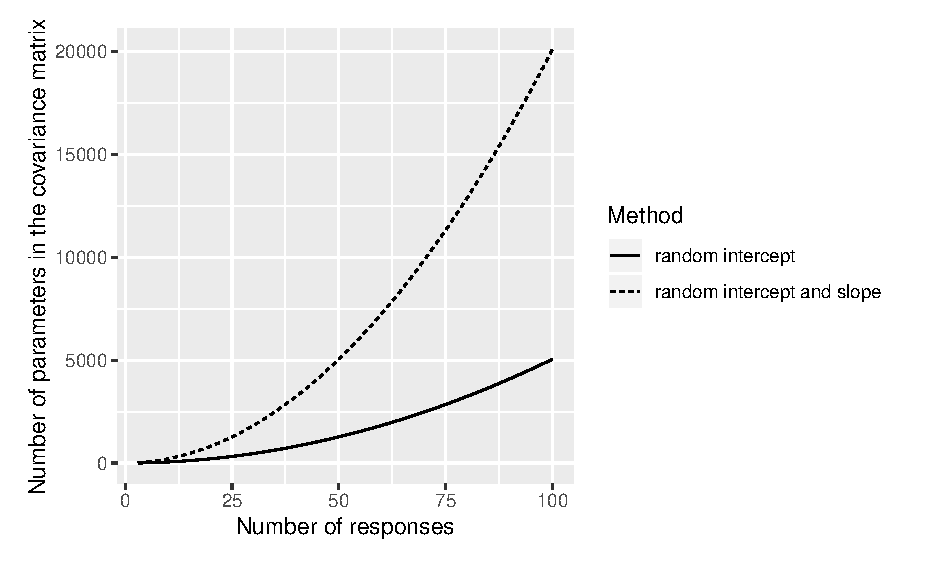
\includegraphics[width=\textwidth]{strucVert.eps}
\caption{Number of parameters in the covariance matrix of jointly normally distributed random effects for different number of responses using only random intercept or random intercept and slope models.} 
\label{fig_strucVert}
\end{figure} 

Therefore, there is a main difference between the applications we have proposed for random vertical splitting, and structured vertical splitting. While both of them are proposed to deal with large clusters, the issue with random vertical splitting is a large sample size, while structured vertical splitting deals with a high-dimensional parameter space. In other words, in case of structured random splitting we are dealing with the so-called curse of dimensionality \citep{donoho2000}. In fact, exactly for this \emph{big} parameter space, we had to impose a structure on it, so in every sub-sample a sub-set of this parameter vector could be estimated. The smart idea of modeling several outcomes by all their sub-sets of two would break down the parameter space by breaking down the sample itself. That is why, in case of random splitting, every sub-sample usually estimates all parameters, while this is not often the case for structured vertical splitting. 

We have two examples in our motivational datasets which are used to illustrate the applications of structured vertical splitting. We have used \emph{Leuven diabetes project} data as a basis to perform simulation studies to evaluate our proposed way of combining variances with what pseudo-likelihood theory would give. Furthermore, the \emph{Hearing data} is used as an example of high-dimensional parameter space where the conventional methods would fail. 


\section{Supplementary topics}

As it was mentioned, due to several technical similarities between random vertical data splitting (iterative multiple outputation) and multiple imputation, and due to wide acceptance of MI in different research fields, we have developed part of our required methodology in MI language rather than language of IMO. However, the conclusions are valid in both cases. In this section we briefly go over these contributions which will be presented in Chapter \textbf{NUMBER OF CHAPTERS}.

\subsection{How many sub-samples?}

The iterative multiple outputation (IMO) procedure that we have proposed for random vertical splitting displays a stopping rule at step 4. This is used to determine the number of sub-samples. Let us briefly explain the idea behind this stopping rule in this section. Obviously, more sub-samples are better in case of obtaining a more precise estimate. But on the other hand, as the sub-samples are with replacement, on can take an infinite number of sub-samples, so there is a need for a rule to stop the IMO procedure. 

As we have seen in (\ref{eq_estimate}), the combination rule of data splitting for parameter estimate is averaging. From laws of large numbers we know that under general regularity conditions, as the sample size increases, the average converges to a finite quantity. We have seen that also via central limit theorem in (\ref{eq_clt_pseudolikelihood}). As we average over sub-samples, sample size here means the number of sub-samples. Therefore, we would expect, after some point, increasing the number of sub-samples would not impressively change the final results. But it is important to come up with appropriate criteria and stopping rule to stop the sub-sampling at the right moment. It is important for two main reasons: 1- if we stop early, we would fail to provide precise and correct estimates, 2- if we stop too late our initial intention for saving computation time could be compromised.

We have already explained the connection of multiple imputation and IMO, also how they would suffer from the same issues. In multiple imputation also, a main issue is to determine the number of imputed datasets. Therefore, we have studied this question in detail via simulation studies and theoretical discussion. Various distance function (Mahalanobis, Euclidean, etc.) were examined for different situations and as a result we proposed the iterative multiple imputation procedure. The obtained results are all valid in case of IMO, therefore, we have used the same stopping rule in IMO and in IMI.

In order to illustrate IMI, we have used two datasets, the \emph{Leuven Eye Study} (LES) and the \emph{Age-related macular degeneration} (ARMD). LES is collected via one of the largest observational studies for glaucoma. However, the dataset includes a lot of missing data. Practically, no fully observed line exists in this dataset, so without MI the analysis was not possible. 

The second dataset, which is also ophthalmology related, come from a clinical trial that tries to compare two methods to diagnose the age related mascular degenaration which causes central vision loss. The final dataset is highly unbalanced, and only includes 17 clusters. \cite{van2016} proposed to make the clusters balanced by imputation them using MI. 

For both of these datasets, determining a correct and sufficient number of imputed datasets is very important, as due to large amount of missing values, as well as small sample size in ARMD, the traditional 5 imputed datasets recipe would not be sufficient. 

\subsection{Special case: where combination rule fails}

A fundamental rule which should be followed when using the combination rule in (\ref{eq_estimate}) is to average parameters which are counterparts of the same parameter in the model for the full sample. In some applications, finding such counter parts is not a straightforward task. An example of such situations is principal component analysis (PCA). Methods like PCA are working based on eigenvalue decomposition of the covariance (or correlation) matrix. Eigenvalues of a matrix $\Sigma$ can be ontained by solving the following equation,

$$|\Sigma-\lambda I|,$$ 

where $|.|$ for a matrix denotes the determinant of it and $I$ is the identity matrix of the same order as $\Sigma$. The roots of this equation are the eigenvalues. Obviously, there is no natural ordering among roots of a polynomial but as in PCA one can show that \citep{mardiamultivariate} these eigenvalues are actually variances of their corresponding principal components, therefore, a PC with a larger eigenvalue explains a larger propportion of variance. 

The issue arises when we use data splitting or multiple imputation where the eigenvalue decomposition should be done for several sub-samples or several imputed datasets. There is no guarantee that the largest eigenvalue from first datasets corresponds to the largest eigenvalue from the second dataset. The problem of combining results of PCA or exploratory factor analysis at the factor (or principal components) level has been studies in \cite{lovik2017combining}. 

Our alternative solution here to first estimate the covariance matrix as out parameter of interest, and then perform the eigenvalue decomposition on this single estimated covariance matrix. We have studied this idea in detail and investigated different aspects of it, also compared it with other alternative solutions. Again, the problem is considered in the setting of multiple imputation, but all the findings are also valid for data splitting. This is because, the issue in this case is that the dataset under study is replaced with several datasets. Now these several datasets could come from data splitting or multiple imputation, that would not change the problem, hence, the proposed solutions.




\section{Software implementation}

Our main concern is R, but for comparison reasons, we have also used SAS.
